\begin{solution}.
The answer to both cases of the problem is equal to $5$.\\[0.2cm]
\noindent \textbf{$6 \times 13$ case}: 
\begin{center}
	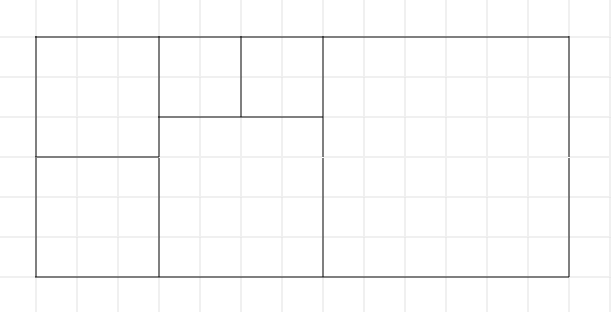
\includegraphics[width=9cm]{47/figs/47_sol1.png}
\end{center}
\noindent \textbf{$9 \times 10$ case}: 
\begin{center}
	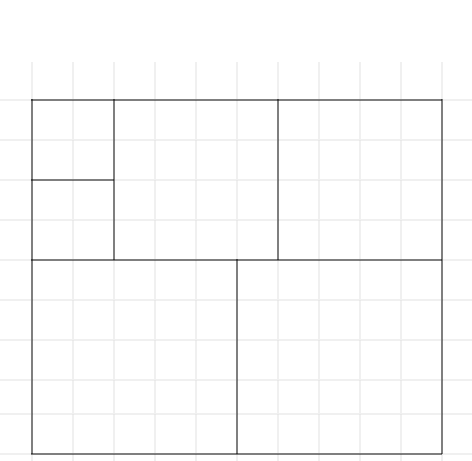
\includegraphics[width=9cm]{47/figs/47_sol2.png}
\end{center}
Below we explain why 5 cuts are necessary in both cases. Keep in mind that the only case where no cut is necessary is when the starting rectangle is already a square. We can solve the problem with one cut only if the starting rectangle has dimensions $(x,2x)$ or $(2x,x)$ for some integer $x$. Also, the only cases where the problem is solvable with two cuts are the ones whose original rectangle has dimensions $(x,1.5x)$ or $(1.5x, x)$ for some even $x$ or dimensions $(x,3x)$ or $(3x,x)$ for some integer $x$. Keep in mind that none of the cases of our problem fall in any of these categories and thus 3 cuts are necessary to cut the original rectangles in each case.

The only way we can solve the problem with 4 cuts is if after the first two cuts, we end up with either (i) two squares and a rectangle that can be divided into squares with 3 cuts or (ii) one square and two rectangles whose dimensions are $(x,2x)$ or $(2x,x)$ and $(y,2y)$ or $(2y,y)$ for some integer $x$ and some integer $y$. Moreover, the total area of these rectangles should be equal to the area of the original rectangle. For the $6 \times 13$ case, there are only two combinations of such rectangles whose total area is $6\cdot 13 = 78$ (we ignore the cases that are identical up to rotation by 90 degrees):
\begin{itemize}
	\item (2, 2), (1, 2), (6, 12),
	\item (6, 6), (6, 6), (2, 3).
\end{itemize} 
Obviously, there is no way to decompose a $6 \times 13$ rectangle into either combination with 2 cuts. Thus we need at least 5 cuts to solve the first problem.

Similarly, there are three such combinations for the $9 \times 10$ case whose total area are equal to $9\cdot 10=90$.
\begin{itemize}
	\item (1,1), (2,2), (3,9)
	\item (4, 4), (1, 2), (6, 12)
	\item (8, 8), (2, 4), (3, 6)
\end{itemize}
Again, none of the combinations is constructable with two cuts starting from a $9 \times 10$ rectangle.
\end{solution}